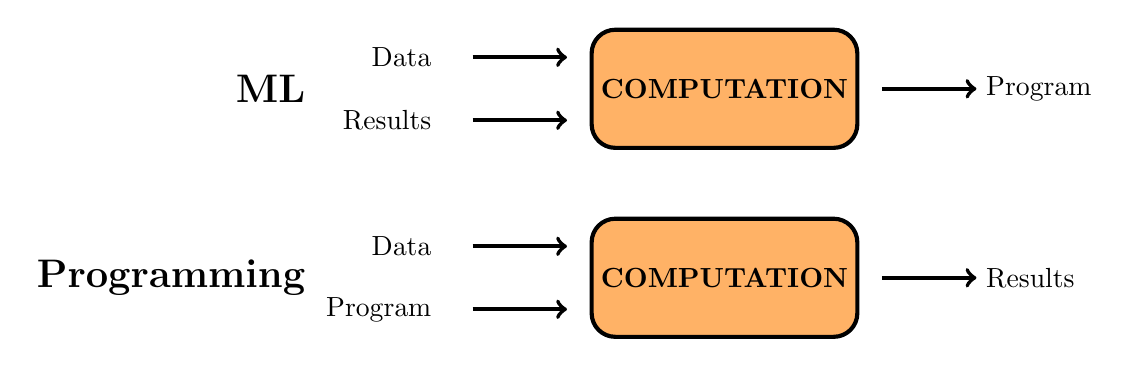
\begin{tikzpicture}[scale=0.8]
  % Styling
  \tikzset{
    box/.style={
      rectangle,
      rounded corners=0.3cm,
      minimum width=3cm,
      minimum height=1.5cm,
      fill=orange!60,
      draw=black,
      line width=1.5pt,
      font=\bfseries
    },
    arrow/.style={
      ->,
      line width=1.5pt,
      black
    },
    label/.style={
      font=\normalsize,
      black
    },
    bigLabel/.style={
      font=\Large\bfseries,
      black
    }
  }
  
  % ===== Machine Learning =====
  \node[bigLabel, left] at (-3, 3) {ML};
  % Input labels
  \node[label, left] at (-1, 3.5) {Data};
  \node[label, left] at (-1, 2.5) {Results};
  
  % Arrows from inputs
  \draw[arrow] (-0.5, 3.5) -- (1, 3.5);
  \draw[arrow] (-0.5, 2.5) -- (1, 2.5);
  
  % Main computation box
  \node[box] (comp1) at (3.5, 3) {COMPUTATION};
  
  % Arrow to output
  \draw[arrow] (6, 3) -- (7.5, 3);
  
  % Output label
  \node[label, right] at (7.5, 3) {Program};
  
  % ===== Programming Approach =====
  \node[bigLabel, left] at (-3, 0) {Programming};
  % Input labels
  \node[label, left] at (-1, 0.5) {Data};
  \node[label, left] at (-1, -0.5) {Program};
  
  % Arrows from inputs
  \draw[arrow] (-0.5, 0.5) -- (1, 0.5);
  \draw[arrow] (-0.5, -0.5) -- (1, -0.5);
  
  % Main computation box
  \node[box] (comp2) at (3.5, 0) {COMPUTATION};
  
  % Arrow to output
  \draw[arrow] (6, 0) -- (7.5, 0);
  
  % Output label
  \node[label, right] at (7.5, 0) {Results};
  
\end{tikzpicture}
